\documentclass[11pt]{article}

% 1. Load the basic TikZ package
\usepackage{tikz}

% 2. Load the OLD arrows library (compatible with CTeX/MiKTeX 2.9)
% Note: We do NOT use arrows.meta here.
\usetikzlibrary{arrows}
\usepackage{listings}   % To display the source code blocks

% 2. Setup the look of the code blocks
\definecolor{codebg}{rgb}{0.97,0.97,0.97}
\definecolor{codegreen}{rgb}{0,0.5,0}
\lstset{
    backgroundcolor=\color{codebg},
    basicstyle=\ttfamily\small,
    breaklines=true,
    commentstyle=\color{codegreen},
    frame=single,
    keywordstyle=\color{blue},
    language=[LaTeX]TeX,
    showstringspaces=false,
    morekeywords={tikzpicture, draw, fill, node}
}

\title{TikZ Coordinate Tutorial (Legacy Version)}
\author{Lei Deng \\ Compatible with TikZ 2.x}
\date{\today}

\begin{document}
\maketitle

\section{Coordinate Systems}
TikZ supports two main ways to define a point:

\begin{itemize}
    \item \textbf{Cartesian:} (x, y) --- e.g., \texttt{(2,1)}
    \item \textbf{Polar:} (angle:distance) --- e.g., \texttt{(30:2cm)}
\end{itemize}

\begin{lstlisting}

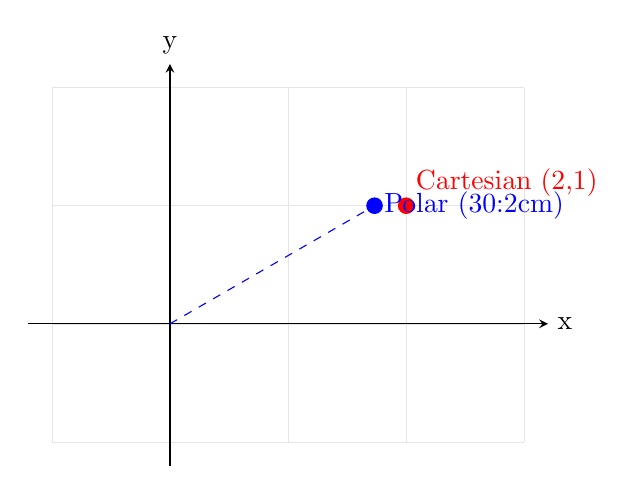
\begin{tikzpicture}[scale=1.5]
    % Draw a background grid
    \draw[gray!20, very thin] (-1,-1) grid (3,2);

    % Draw Axes using standard arrows
    % Syntax: [->] is a standard arrow. [>=stealth] sets the tip style.
    \draw[->, >=stealth] (-1.2,0) -- (3.2,0) node[right] {x};
    \draw[->, >=stealth] (0,-1.2) -- (0,2.2) node[above] {y};

    % Cartesian Point
    \fill[red] (2,1) circle (2pt);
    \node[red, anchor=south west] at (2,1) {Cartesian (2,1)};

    % Polar Point (30 degrees, 2cm away)
    \draw[blue, dashed] (0,0) -- (30:2);
    \fill[blue] (30:2) circle (2pt);
    \node[blue, anchor=west] at (30:2) {Polar (30:2cm)};
\end{tikzpicture}
\end{lstlisting}

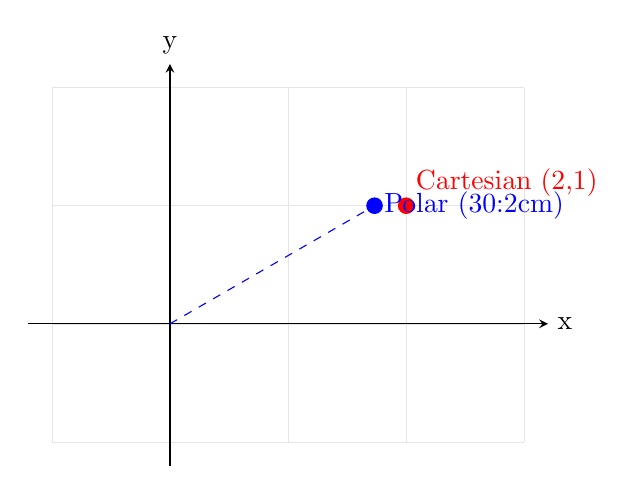
\begin{tikzpicture}[scale=1.5]
    % Draw a background grid
    \draw[gray!20, very thin] (-1,-1) grid (3,2);

    % Draw Axes using standard arrows
    % Syntax: [->] is a standard arrow. [>=stealth] sets the tip style.
    \draw[->, >=stealth] (-1.2,0) -- (3.2,0) node[right] {x};
    \draw[->, >=stealth] (0,-1.2) -- (0,2.2) node[above] {y};

    % Cartesian Point
    \fill[red] (2,1) circle (2pt);
    \node[red, anchor=south west] at (2,1) {Cartesian (2,1)};

    % Polar Point (30 degrees, 2cm away)
    \draw[blue, dashed] (0,0) -- (30:2);
    \fill[blue] (30:2) circle (2pt);
    \node[blue, anchor=west] at (30:2) {Polar (30:2cm)};
\end{tikzpicture}

\newpage

\section{Relative Coordinates: ++ vs +}
This is the most important concept for drawing paths.

\begin{itemize}
    \item \textbf{++ (Cumulative):} Moves the "pen" to the new location.
    \item \textbf{+ (Non-cumulative):} Draws to the point but returns the "pen" to the previous location.
\end{itemize}

\begin{lstlisting}

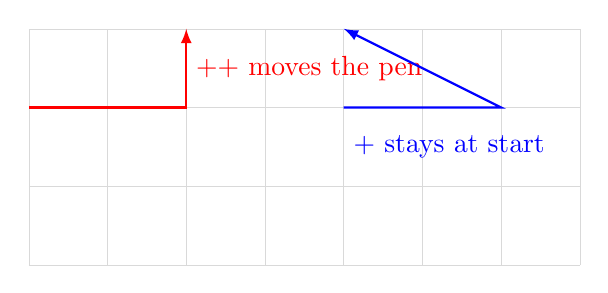
\begin{tikzpicture}[scale=1]
    \draw[help lines, gray!30] (0,0) grid (7,3);

    % Example of ++
    % Starts at (0,2), moves 2 right, then moves 1 up FROM THERE.
    \draw[thick, red, ->, >=latex] (0,2) -- ++(2,0) -- ++(0,1);
    \node[red, right] at (2,2.5) {++ moves the pen};

    % Example of +
    % Starts at (4,2), draws to (4+2, 2), then draws to (4, 2+1).
    \draw[thick, blue, ->, >=latex] (4,2) -- +(2,0) -- +(0,1);
    \node[blue, right] at (4,1.5) {+ stays at start};
\end{tikzpicture}

\end{lstlisting}


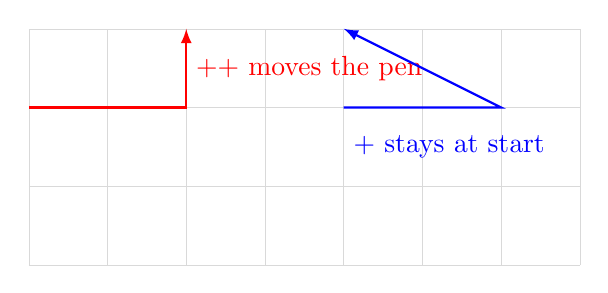
\begin{tikzpicture}[scale=1]
    \draw[help lines, gray!30] (0,0) grid (7,3);

    % Example of ++
    % Starts at (0,2), moves 2 right, then moves 1 up FROM THERE.
    \draw[thick, red, ->, >=latex] (0,2) -- ++(2,0) -- ++(0,1);
    \node[red, right] at (2,2.5) {++ moves the pen};

    % Example of +
    % Starts at (4,2), draws to (4+2, 2), then draws to (4, 2+1).
    \draw[thick, blue, ->, >=latex] (4,2) -- +(2,0) -- +(0,1);
    \node[blue, right] at (4,1.5) {+ stays at start};
\end{tikzpicture}

\newpage

\section{Node Anchors}
Nodes have "sticky" points called anchors. You can use these to connect lines precisely.

\begin{lstlisting}


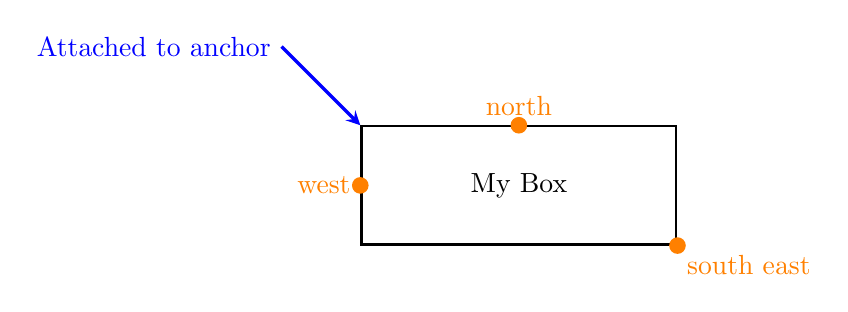
\begin{tikzpicture}
    % Define a node
    \node[draw, minimum width=4cm, minimum height=1.5cm, thick] (Box) at (0,0) {My Box};

    % Draw points at specific anchors
    \fill[orange] (Box.north) circle (3pt) node[above] {north};
    \fill[orange] (Box.south east) circle (3pt) node[below right] {south east};
    \fill[orange] (Box.west) circle (3pt) node[left] {west};

    % Connect a line to an anchor using old arrow syntax
    % In old TikZ, arrow names are lowercase: stealth, latex, to
    \draw[<-, >=stealth, blue, very thick] (Box.north west) -- ++(-1,1) node[left] {Attached to anchor};
\end{tikzpicture}


\end{lstlisting}



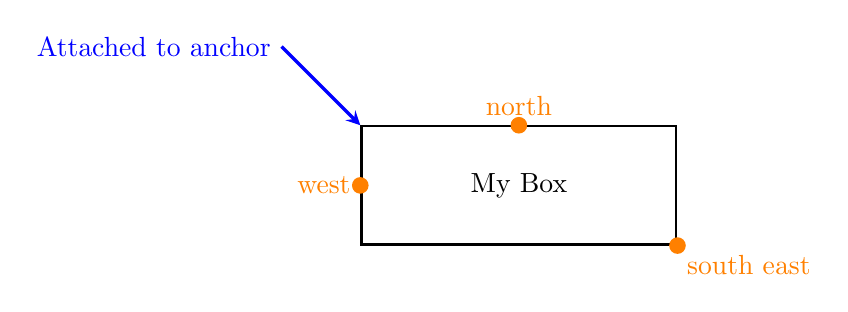
\begin{tikzpicture}
    % Define a node
    \node[draw, minimum width=4cm, minimum height=1.5cm, thick] (Box) at (0,0) {My Box};

    % Draw points at specific anchors
    \fill[orange] (Box.north) circle (3pt) node[above] {north};
    \fill[orange] (Box.south east) circle (3pt) node[below right] {south east};
    \fill[orange] (Box.west) circle (3pt) node[left] {west};

    % Connect a line to an anchor using old arrow syntax
    % In old TikZ, arrow names are lowercase: stealth, latex, to
    \draw[<-, >=stealth, blue, very thick] (Box.north west) -- ++(-1,1) node[left] {Attached to anchor};
\end{tikzpicture}

\newpage

\section{Common Old-Style Arrows}
Here are the arrow types available in your version:

\begin{lstlisting}

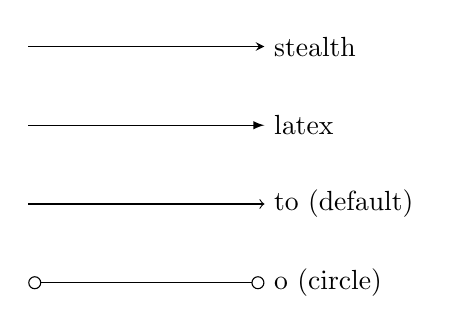
\begin{tikzpicture}
    \draw[->, >=stealth] (0,3) -- (3,3) node[right] {stealth};
    \draw[->, >=latex]   (0,2) -- (3,2) node[right] {latex};
    \draw[->, >=to]      (0,1) -- (3,1) node[right] {to (default)};
    \draw[<->, >=o]      (0,0) -- (3,0) node[right] {o (circle)};
\end{tikzpicture}


\end{lstlisting}

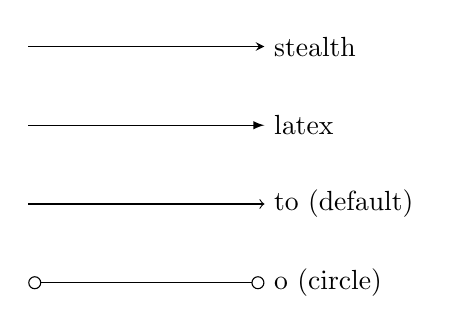
\begin{tikzpicture}
    \draw[->, >=stealth] (0,3) -- (3,3) node[right] {stealth};
    \draw[->, >=latex]   (0,2) -- (3,2) node[right] {latex};
    \draw[->, >=to]      (0,1) -- (3,1) node[right] {to (default)};
    \draw[<->, >=o]      (0,0) -- (3,0) node[right] {o (circle)};
\end{tikzpicture}

\end{document}